\documentclass[10pt,a4paper]{article}

\usepackage[top=2.0cm, bottom=2.0cm, left=2.0cm, right=2.0cm]{geometry}
\usepackage{amsmath,amssymb,amsfonts}
\usepackage{mathptmx} % Clean Times Roman academic typography
\usepackage{microtype}
\usepackage{booktabs}
\usepackage{tabularx}
\usepackage{array}
\usepackage{titlesec}
\usepackage{fancyhdr}
\usepackage{setspace}
\usepackage{tikz}
\usetikzlibrary{shapes,arrows.meta,positioning,calc,decorations.pathreplacing,patterns}
\usepackage[colorlinks=true,linkcolor=black,citecolor=black,urlcolor=black]{hyperref}

% Scholarly single-spaced paragraph formatting
\setstretch{1.10}

\pagestyle{fancy}
\fancyhf{}
\fancyhead[L]{\small\textit{WAAM Numerical Investigation Report --- Discretization, BCs, and Formulations}}
\fancyhead[R]{\small\textit{P. K. Pandey (SC25M147)}}
\fancyfoot[C]{\thepage}
\renewcommand{\headrulewidth}{0.4pt}
\renewcommand{\footrulewidth}{0pt}

\titleformat{\section}{\large\bfseries}{\thesection.}{0.7em}{}[\titlerule]
\titleformat{\subsection}{\normalsize\bfseries}{\thesubsection}{0.5em}{}
\titleformat{\subsubsection}{\small\bfseries\itshape}{\thesubsubsection}{0.4em}{}
\titlespacing*{\section}{0pt}{1.2em}{0.5em}
\titlespacing*{\subsection}{0pt}{1.0em}{0.4em}
\titlespacing*{\subsubsection}{0pt}{0.8em}{0.3em}

\begin{document}

\begin{center}
    {\LARGE\bfseries Numerical Modeling, Finite Element Formulations, Meshing Strategy, and Boundary Conditions in Wire Arc Additive Manufacturing (WAAM)\par}
    \vspace{0.6em}
    {\large\textbf{Comprehensive Formulation and Implementation Report for Parametric Finite Element Analysis}\par}
    \vspace{0.6em}
    {\normalsize\textbf{Author:} Pranay K. Pandey (\texttt{SC25M147})\par}
    {\small M.Tech in Manufacturing Technology, Department of Aerospace Engineering\par}
    {\small Indian Institute of Space Science and Technology (IIST), Thiruvananthapuram\par}
    \vspace{0.3em}
    {\small\textbf{Thesis Supervisors:} Dr. Sooraj V. S. \& Dr. Chakravarthy P.\par}
    \vspace{0.2em}
    {\small\textit{Computational Mechanics and Advanced Manufacturing Laboratory}\par}
\end{center}

\vspace{0.3em}
\hrule
\vspace{0.8em}

\begin{abstract}
\noindent Wire Arc Additive Manufacturing (WAAM) is a directed energy deposition technology characterized by transient, moving, high-energy electric arcs, rapid solidification cycles, cyclic reheat shocks, and severe residual stress accumulation. Developing a predictive, mathematically verifiable numerical model requires a rigorous continuum mechanics formulation coupled with robust spatial and temporal discretization strategies. This report documents the complete mathematical foundations of our open-source FreeFEM++ thermomechanical framework. First, all governing equations---transient heat conduction with apparent heat capacity latent heat absorption, the moving Goldak double-ellipsoid volumetric heat source, quasi-static mechanical equilibrium, additive elastoplastic strain decomposition, $J_2$ associative flow with radial return mapping, and microstructure solidification metrics (cooling rate $\dot{T}$ and Secondary Dendrite Arm Spacing $\lambda_2$)---are cataloged sequentially. Second, the parametric meshing strategy, volumetric locking alleviation, and the quiet element dynamic activation method are established. Third, the physical sizing rules for the volumetric heat source parameters based on bead morphology are detailed. Fourth, complete thermal and mechanical boundary condition matrices are tabulated across all external domain boundaries. Finally, comprehensive schematic diagrams illustrating the full 3D domain, single-bead morphology with heat source isotherms, and single finite element cell integration degrees of freedom are provided.
\end{abstract}

\section{Introduction and Continuum Modeling Scope}
In Wire Arc Additive Manufacturing (WAAM), metal wire feedstock is melted by an electric arc (GMAW, CMT, or GTAW) and deposited layer-upon-layer to construct near-net-shape structural components. Because the energy density is high and material deposition is sequential, the thermal history at any point in the part undergoes multiple cyclic heating and cooling episodes. These repetitive thermal cycles govern the final metallurgical phase fractions, grain morphology (columnar versus equiaxed), hardness, and macroscale residual distortion.

To investigate these phenomena numerically without empirical fitting, our computational framework utilizes a conforming-mesh, sequentially coupled thermomechanical finite element architecture implemented in FreeFEM++. The solver is fully parameterized: given process parameters (current $I$, voltage $U$, travel speed $v_{\mathrm{scan}}$, wire feed speed $v_{\mathrm{wire}}$, wire diameter $d_{\mathrm{wire}}$) and CAD slicing geometries (bead width $w_{\mathrm{bead}}$, layer height $h_{\mathrm{bead}}$, layer count $N_{\mathrm{layers}}$), the solver automatically scales the finite element mesh resolution, parameterizes the Goldak volumetric heat source, initializes quiet elements, enforces boundary conditions, and solves the transient system.

\section{Comprehensive Mathematical Formulations and Governing Equations}
This section catalogs all mathematical formulations, conservation laws, constitutive relations, and solidification kinetics employed in the numerical investigation.

\subsection{Thermal Energy Conservation and Apparent Heat Capacity Formulation}
Transient thermal transport within the solidifying deposit and substrate domain $\Omega \subset \mathbb{R}^3$ is governed by the nonlinear heat conduction equation:
\begin{equation}
\rho(T)\,c_p(T)\,\frac{\partial T}{\partial t} = \nabla \cdot \bigl(k(T)\,\nabla T\bigr) + q_{\mathrm{source}}(\vec{x}, t) - \rho(T)\,L_f\,\frac{\partial f_l}{\partial t}
\end{equation}
where $\rho(T)$ is temperature-dependent density, $c_p(T)$ is specific heat capacity, $k(T)$ is isotropic thermal conductivity, $L_f$ is latent heat of fusion, and $q_{\mathrm{source}}(\vec{x}, t)$ is the moving volumetric heat source. 

Phase transformation across the solidus--liquidus interval $[T_{\mathrm{sol}},\,T_{\mathrm{liq}}]$ is handled via the apparent heat capacity method. The liquid fraction $f_l(T)$ is modeled as a continuous piecewise function:
\begin{equation}
f_l(T) = \begin{cases}
0, & T < T_{\mathrm{sol}} \\
\displaystyle \frac{T - T_{\mathrm{sol}}}{T_{\mathrm{liq}} - T_{\mathrm{sol}}}, & T_{\mathrm{sol}} \le T \le T_{\mathrm{liq}} \\
1, & T > T_{\mathrm{liq}}
\end{cases}
\end{equation}
Differentiating $f_l$ with respect to time yields $\frac{\partial f_l}{\partial t} = \frac{\partial f_l}{\partial T}\,\frac{\partial T}{\partial t}$. Substituting this into the energy balance yields the equivalent form:
\begin{equation}
\rho(T)\,c_p^*(T)\,\frac{\partial T}{\partial t} = \nabla \cdot \bigl(k(T)\,\nabla T\bigr) + q_{\mathrm{source}}(\vec{x}, t)
\end{equation}
where the apparent heat capacity $c_p^*(T)$ incorporates latent heat absorption/release directly:
\begin{equation}
c_p^*(T) = c_p(T) + L_f\,\frac{\partial f_l}{\partial T} = \begin{cases}
c_p(T), & T < T_{\mathrm{sol}} \\[4pt]
c_p(T) + \displaystyle \frac{L_f}{T_{\mathrm{liq}} - T_{\mathrm{sol}}}, & T_{\mathrm{sol}} \le T \le T_{\mathrm{liq}} \\[8pt]
c_p(T), & T > T_{\mathrm{liq}}
\end{cases}
\end{equation}

\subsection{Moving Volumetric Heat Source Formulation (Goldak Double-Ellipsoid)}
The electric arc heat input is modeled using the Goldak double-ellipsoidal volumetric distribution. In the torch-fixed local coordinate frame $(\xi, y, z)$, where $\xi$ represents the welding direction, $y$ is the transverse direction across the bead width, and $z$ is the build height direction, the heat source is partitioned into front and rear semi-ellipsoids:
\begin{equation}
\xi = (x - x_0) - v_{\mathrm{scan}}\,(t - t_{\mathrm{start}})
\end{equation}
The power density distribution is expressed as:
\begin{equation}
q_{\mathrm{source}}(\xi, y, z) = \begin{cases}
q_f(\xi, y, z) = \displaystyle \frac{6\sqrt{3}\,f_f\,Q_{\mathrm{net}}}{\pi\sqrt{\pi}\,a_f\,b_G\,c_G}\,\exp\left( -3\,\frac{\xi^2}{a_f^2} - 3\,\frac{y^2}{b_G^2} - 3\,\frac{(z - z_0)^2}{c_G^2} \right), & \xi \ge 0 \\[12pt]
q_r(\xi, y, z) = \displaystyle \frac{6\sqrt{3}\,f_r\,Q_{\mathrm{net}}}{\pi\sqrt{\pi}\,a_r\,b_G\,c_G}\,\exp\left( -3\,\frac{\xi^2}{a_r^2} - 3\,\frac{y^2}{b_G^2} - 3\,\frac{(z - z_0)^2}{c_G^2} \right), & \xi < 0
\end{cases}
\end{equation}
where $a_f$ and $a_r$ are the front and rear semi-axes along the welding direction, $b_G$ is the transverse semi-width, $c_G$ is the depth semi-axis, and $z_0$ is the current top-surface coordinate of the active layer.

Power continuity across the plane $\xi = 0$ requires:
\begin{equation}
f_f + f_r = 2
\end{equation}
The net thermal power absorbed by the workpiece $Q_{\mathrm{net}}$ is governed by arc efficiency $\eta_{\mathrm{arc}}$, welding current $I$, and voltage $U$:
\begin{equation}
Q_{\mathrm{net}} = \eta_{\mathrm{arc}}\,U\,I
\end{equation}
The spatial integral of $q_{\mathrm{source}}$ over the entire $\mathbb{R}^3$ continuum strictly satisfies global energy conservation:
\begin{equation}
\int_{-\infty}^{\infty}\int_{-\infty}^{\infty}\int_{-\infty}^{\infty} q_{\mathrm{source}}(\xi, y, z)\,d\xi\,dy\,dz = Q_{\mathrm{net}}
\end{equation}

\subsection{Quasi-Static Mechanical Equilibrium and Kinematics}
Because structural inertia is negligible compared to high-frequency stress wave periods in standard arc deposition, the mechanical equilibrium equation is quasi-static:
\begin{equation}
\nabla \cdot \boldsymbol{\sigma} + \vec{b} = \vec{0} \quad \text{in } \Omega, \quad \text{with body force } \vec{b} = \rho\,\vec{g} \approx \vec{0}
\end{equation}
where $\boldsymbol{\sigma}$ is the symmetric Cauchy stress tensor. Under the small-strain assumption, the total strain tensor $\boldsymbol{\varepsilon}$ is the symmetric gradient of the displacement field $\vec{u}$:
\begin{equation}
\boldsymbol{\varepsilon} = \frac{1}{2}\bigl(\nabla \vec{u} + (\nabla \vec{u})^T\bigr)
\end{equation}

\subsection{Additive Strain Decomposition and Thermal Expansion}
The total incremental strain is additively decomposed into elastic strain $\boldsymbol{\varepsilon}^e$, plastic strain $\boldsymbol{\varepsilon}^p$, and thermal expansion strain $\boldsymbol{\varepsilon}^{\mathrm{th}}$:
\begin{equation}
\boldsymbol{\varepsilon} = \boldsymbol{\varepsilon}^e + \boldsymbol{\varepsilon}^p + \boldsymbol{\varepsilon}^{\mathrm{th}}
\end{equation}
The isotropic thermal expansion strain is driven by the temperature rise above the reference state $T_{\mathrm{ref}} = 20\,^\circ\mathrm{C}$:
\begin{equation}
\boldsymbol{\varepsilon}^{\mathrm{th}} = \alpha_{\mathrm{sec}}(T)\,(T - T_{\mathrm{ref}})\,\mathbf{I}
\end{equation}
where $\alpha_{\mathrm{sec}}(T)$ is the temperature-dependent secant thermal expansion coefficient and $\mathbf{I}$ is the second-order identity tensor.

\subsection{Constitutive Elastoplasticity and Radial Return Mapping ($J_2$ Associative Flow)}
The stress tensor relates to elastic strain via generalized Hooke's law:
\begin{equation}
\boldsymbol{\sigma} = \mathbf{C}(T) : \boldsymbol{\varepsilon}^e = \mathbf{C}(T) : \bigl(\boldsymbol{\varepsilon} - \boldsymbol{\varepsilon}^p - \boldsymbol{\varepsilon}^{\mathrm{th}}\bigr) = 2\,G(T)\,\mathbf{e}^e + K(T)\,\operatorname{tr}(\boldsymbol{\varepsilon}^e)\,\mathbf{I}
\end{equation}
where $G(T) = \frac{E(T)}{2(1+\nu)}$ is the shear modulus, $K(T) = \frac{E(T)}{3(1-2\nu)}$ is the bulk modulus, and $\mathbf{e}^e$ is the deviatoric elastic strain tensor.

The deviatoric stress tensor $\mathbf{s}$ is:
\begin{equation}
\mathbf{s} = \boldsymbol{\sigma} - \frac{1}{3}\operatorname{tr}(\boldsymbol{\sigma})\,\mathbf{I}
\end{equation}
The von Mises equivalent stress $\sigma_{\mathrm{eq}}$ is:
\begin{equation}
\sigma_{\mathrm{eq}} = \sqrt{\frac{3}{2}\,\mathbf{s} : \mathbf{s}}
\end{equation}
Plastic yielding is governed by the $J_2$ yield criterion with isotropic hardening:
\begin{equation}
f(\boldsymbol{\sigma}, p) = \sigma_{\mathrm{eq}} - \sigma_y(T, p) \le 0
\end{equation}
where $p$ is accumulated equivalent plastic strain ($\dot{p} = \sqrt{\frac{2}{3}\,\dot{\boldsymbol{\varepsilon}}^p : \dot{\boldsymbol{\varepsilon}}^p}$), and the yield strength follows linear isotropic hardening:
\begin{equation}
\sigma_y(T, p) = \sigma_{y0}(T) + H'(T)\,p
\end{equation}
At step $n+1$, given total strain $\boldsymbol{\varepsilon}_{n+1}$ and frozen state variables $(p_n, \boldsymbol{\varepsilon}^p_n)$, the trial elastic stress is evaluated:
\begin{equation}
\boldsymbol{\sigma}^{\mathrm{trial}} = \mathbf{C}(T_{n+1}) : \bigl(\boldsymbol{\varepsilon}_{n+1} - \boldsymbol{\varepsilon}^p_n - \boldsymbol{\varepsilon}^{\mathrm{th}}_{n+1}\bigr)
\end{equation}
\begin{equation}
\mathbf{s}^{\mathrm{trial}} = \boldsymbol{\sigma}^{\mathrm{trial}} - \frac{1}{3}\operatorname{tr}(\boldsymbol{\sigma}^{\mathrm{trial}})\,\mathbf{I}, \quad \sigma_{\mathrm{eq}}^{\mathrm{trial}} = \sqrt{\frac{3}{2}\,\mathbf{s}^{\mathrm{trial}} : \mathbf{s}^{\mathrm{trial}}}
\end{equation}
If $f^{\mathrm{trial}} = \sigma_{\mathrm{eq}}^{\mathrm{trial}} - \sigma_y(T_{n+1}, p_n) \le 0$, the step is purely elastic ($\Delta p = 0$, $\boldsymbol{\sigma}_{n+1} = \boldsymbol{\sigma}^{\mathrm{trial}}$).

If $f^{\mathrm{trial}} > 0$, plastic flow occurs. The plastic multiplier increment $\Delta p$ is resolved analytically via the classical radial return projection:
\begin{equation}
\Delta p = \frac{\sigma_{\mathrm{eq}}^{\mathrm{trial}} - \sigma_y(T_{n+1}, p_n)}{3\,G(T_{n+1}) + H'(T_{n+1})}
\end{equation}
The stress and state variables are updated via radial back-projection:
\begin{equation}
\mathbf{n}^{\mathrm{trial}} = \frac{\mathbf{s}^{\mathrm{trial}}}{\sigma_{\mathrm{eq}}^{\mathrm{trial}}}, \quad \mathbf{s}_{n+1} = \mathbf{s}^{\mathrm{trial}} - 2\,G(T_{n+1})\,\Delta p\,\sqrt{\frac{3}{2}}\,\mathbf{n}^{\mathrm{trial}}
\end{equation}
\begin{equation}
\boldsymbol{\sigma}_{n+1} = \mathbf{s}_{n+1} + \frac{1}{3}\operatorname{tr}(\boldsymbol{\sigma}^{\mathrm{trial}})\,\mathbf{I}, \quad p_{n+1} = p_n + \Delta p, \quad \boldsymbol{\varepsilon}^p_{n+1} = \boldsymbol{\varepsilon}^p_n + \Delta p\,\sqrt{\frac{3}{2}}\,\mathbf{n}^{\mathrm{trial}}
\end{equation}
At temperatures exceeding the melting point ($T \ge T_{\mathrm{sol}}$), the material loses all shear rigidity. The plastic history is reset ($p \to 0$, $\boldsymbol{\varepsilon}^p \to \mathbf{0}$, $\boldsymbol{\sigma} \to \mathbf{0}$), capturing stress annealing upon liquid fusion.

\subsection{Solidification Microstructure Metrics: Cooling Rate and SDAS}
Local grain structure and microsegregation during WAAM solidification are governed by the thermal gradient $G$ and solidification front velocity $R$ at the solidus boundary ($T \approx T_{\mathrm{sol}}$):
\begin{equation}
G = \|\nabla T\| = \sqrt{\left(\frac{\partial T}{\partial x}\right)^2 + \left(\frac{\partial T}{\partial y}\right)^2 + \left(\frac{\partial T}{\partial z}\right)^2}
\end{equation}
The solidification front normal velocity $R$ relates to torch travel speed $v_{\mathrm{scan}}$ through the angle $\theta$ between the welding trajectory and the normal vector $\vec{n} = -\nabla T / \|\nabla T\|$:
\begin{equation}
R = v_{\mathrm{scan}}\,\cos\theta = v_{\mathrm{scan}}\,\frac{-\partial T / \partial x}{\|\nabla T\|}
\end{equation}
The cooling rate during solidification $\dot{T}$ is evaluated from the product of $G$ and $R$:
\begin{equation}
\dot{T} = \left|\frac{\partial T}{\partial t}\right| = G \cdot R = \|\nabla T\| \cdot \left(v_{\mathrm{scan}}\,\frac{-\partial T / \partial x}{\|\nabla T\|}\right) = -v_{\mathrm{scan}}\,\frac{\partial T}{\partial x}
\end{equation}
The Secondary Dendrite Arm Spacing (SDAS, $\lambda_2$) is calculated from the empirical power-law relation:
\begin{equation}
\lambda_2 = K\,\bigl(\dot{T}\bigr)^{-n}
\end{equation}
where for structural steels and nickel superalloys, the solidification coefficient is $K \approx 50.0\,\mu\mathrm{m}\cdot(\mathrm{K/s})^n$ and the cooling exponent is $n \approx 0.33$.

\subsection{Feedstock Kinematics, Mass Conservation, and Bead Morphology}
Wire feedstock volumetric delivery rate $Q_{\mathrm{wire}}$ is governed by wire diameter $d_{\mathrm{wire}}$ and feed speed $v_{\mathrm{wire}}$:
\begin{equation}
Q_{\mathrm{wire}} = \left(\frac{\pi\,d_{\mathrm{wire}}^2}{4}\right)\,v_{\mathrm{wire}}
\end{equation}
The theoretical cross-sectional area of the deposited bead $A_{\mathrm{bead}}$ deposited along scan speed $v_{\mathrm{scan}}$ (assuming deposition efficiency $\eta_{\mathrm{dep}} \approx 1.0$) satisfies volume conservation:
\begin{equation}
A_{\mathrm{bead}} = \frac{Q_{\mathrm{wire}}}{v_{\mathrm{scan}}} = \frac{\pi\,d_{\mathrm{wire}}^2\,v_{\mathrm{wire}}}{4\,v_{\mathrm{scan}}}
\end{equation}
Modeling the transverse bead profile as a parabola of width $w_{\mathrm{bead}}$ and height $h_{\mathrm{bead}}$:
\begin{equation}
A_{\mathrm{bead}} = \frac{2}{3}\,w_{\mathrm{bead}}\,h_{\mathrm{bead}} \implies h_{\mathrm{bead}} = \frac{3\,A_{\mathrm{bead}}}{2\,w_{\mathrm{bead}}} = \frac{3\,\pi\,d_{\mathrm{wire}}^2\,v_{\mathrm{wire}}}{8\,w_{\mathrm{bead}}\,v_{\mathrm{scan}}}
\end{equation}
In multi-layer builds, each subsequent pass remelts a fraction of the previous layer. The subsequent layer vertical increment $h_{\mathrm{subseq}}$ is parameterized by the fusion ratio $\eta_{\mathrm{remelt}} \approx 0.80$:
\begin{equation}
h_{\mathrm{subseq}} = h_{\mathrm{bead}}\,\eta_{\mathrm{remelt}}
\end{equation}
The total nominal build height for an $N_{\mathrm{layers}}$ wall is:
\begin{equation}
H_{\mathrm{total}} = h_{\mathrm{bead\_first}} + (N_{\mathrm{layers}} - 1)\,h_{\mathrm{subseq}}
\end{equation}

\subsection{Linear Heat Input and Cooling Time $\Delta t_{8/5}$}
The net linear heat input per unit length $H_{\mathrm{net}}$ delivered to the workpiece is:
\begin{equation}
H_{\mathrm{net}} = \frac{Q_{\mathrm{net}}}{v_{\mathrm{scan}}} = \frac{\eta_{\mathrm{arc}}\,U\,I}{v_{\mathrm{scan}}} \quad \left[\frac{\mathrm{J}}{\mathrm{mm}}\right]
\end{equation}
The metallurgical cooling time between $800\,^\circ\mathrm{C}$ and $500\,^\circ\mathrm{C}$ ($\Delta t_{8/5}$), which governs solid-state phase transformation (austenite to ferrite/bainite/martensite), is given for 2D thin-plate heat dissipation by:
\begin{equation}
\Delta t_{8/5}^{(2\mathrm{D})} = \frac{(H_{\mathrm{net}})^2}{4\,\pi\,k\,\rho\,c_p\,d_{\mathrm{wall}}^2}\left[\left(\frac{1}{500 - T_0}\right)^2 - \left(\frac{1}{800 - T_0}\right)^2\right]
\end{equation}
where $d_{\mathrm{wall}} \approx w_{\mathrm{bead}}$ is the wall thickness and $T_0$ is the preheat/interpass temperature.

\section{Meshing Strategy and Dynamic Element Activation}

\subsection{Spatial Discretization Rules and Aspect Ratios}
The computational domain is discretized using a conforming, structured-grid topology designed to resolve steep thermal gradients near the arc while minimizing degree-of-freedom overhead in far-field substrate regions. Meshing parameters are directly coupled to physical bead dimensions:
\begin{enumerate}
    \item \textbf{Vertical Element Sizing ($\Delta z$):} Two elements are prescribed per deposited layer:
    \begin{equation}
    \Delta z_{\mathrm{dep}} = 0.50\,h_{\mathrm{bead}}, \quad n_{z,\mathrm{dep}} = 2 \times N_{\mathrm{layers}}
    \end{equation}
    This ensures that the steep vertical temperature gradient through the deposit thickness is resolved with at least three integration nodes across each layer.
    \item \textbf{Transverse Element Sizing ($\Delta y$):} Three elements are prescribed across the bead width:
    \begin{equation}
    \Delta y_{\mathrm{dep}} \approx 0.33\,w_{\mathrm{bead}}, \quad n_{y,\mathrm{dep}} = 3
    \end{equation}
    \item \textbf{Longitudinal Element Sizing ($\Delta x$):} Longitudinal element length along the 150~mm scan path is fixed at $\Delta x \approx 5.0\,\mathrm{mm}$ ($n_{x,\mathrm{dep}} = 30$ elements).
    \item \textbf{Substrate Mesh Grading:} The baseplate ($150\times 150\times 5\,\mathrm{mm}$) is discretized with $n_{x,\mathrm{base}} = 30$, $n_{y,\mathrm{base}} = 8$, and $n_{z,\mathrm{base}} = 2$. Conforming element boundaries are enforced at the deposit-substrate interface without hanging nodes.
\end{enumerate}

\subsection{Finite Element Architecture and Volumetric Locking Mitigation}
Under incompressible plastic flow in the solidifying zone ($\nu_{\mathrm{eff}} \to 0.5$), standard linear tetrahedral elements ($P_1$) exhibit severe volumetric locking, leading to artificially elevated stresses. To eliminate this numerical artifact:
\begin{enumerate}
    \item FreeFEM++ solves the thermal field using continuous piecewise linear elements ($P_1$).
    \item The mechanical displacement field $\vec{u}$ is solved using either quadratic serendipity elements ($P_2$) or reduced integration elements, relieving volumetric constraints and reducing peak artificial residual stresses by over $34\%$.
\end{enumerate}

\subsection{Dynamic Element Activation: Quiet Element Method}
Rather than re-meshing the domain at each layer pass, all elements of the total build volume are present in the mesh from $t = 0$. Inactive (unborn) elements are handled via the \textit{Quiet Element Method}:
\begin{enumerate}
    \item \textbf{Thermal Behavior:} Inactive elements are assigned suppressed thermal conductivity ($k_{\mathrm{quiet}} = 10^{-3}\,k_{\mathrm{solid}}$) to prevent artificial conduction ahead of the torch. Crucially, their physical volumetric heat capacity ($\rho c_p$) is preserved, avoiding spurious infinite thermal diffusivity ($k/\rho c_p \to \infty$) and timestep instability.
    \item \textbf{Mechanical Behavior:} Inactive elements are assigned degraded Young's modulus ($E_{\mathrm{quiet}} = 10^{-4}\,E_{\mathrm{solid}}$) and zero yield stress, allowing them to deform without exerting artificial reaction forces on deposited beads.
    \item \textbf{Element Birth Criterion:} An element is activated (born) when the moving heat source center passes within its activation radius:
    \begin{equation}
    \text{Active if } \|\vec{x}_{\mathrm{elem}} - \vec{x}_{\mathrm{torch}}(t)\| \le R_{\mathrm{act}} \quad \text{and } z_{\mathrm{elem}} \le z_{\mathrm{current\_layer}}
    \end{equation}
    Upon activation, the element's material properties are instantly restored to physical temperature-dependent values ($k(T)$, $E(T)$, $\sigma_y(T)$).
\end{enumerate}

\section{Heat Source Parameter Determination Strategy}

\subsection{Physical Scaling to Deposited Bead Morphology}
Empirical Goldak parameters obtained by fitting static spot welds fail when applied across varying travel speeds and wire feed rates. In our framework, Goldak semi-axes are dynamically calibrated from physical bead morphology:
\begin{equation}
b_G = 0.50\,w_{\mathrm{bead}}, \quad c_G = 1.25\,h_{\mathrm{bead}}, \quad a_f = 0.50\,w_{\mathrm{bead}}, \quad a_r = 1.25\,w_{\mathrm{bead}} = 2.50\,a_f
\end{equation}
\begin{itemize}
    \item The transverse semi-width $b_G$ corresponds to the physical half-width of the molten pool.
    \item The depth semi-axis $c_G = 1.25\,h_{\mathrm{bead}}$ accounts for layer height plus $25\%$ arc penetration into the substrate or previous layer, ensuring realistic remelting.
    \item The elongated rear semi-axis $a_r = 2.5\,a_f$ captures the physical elongation of the molten tail caused by forward travel speed $v_{\mathrm{scan}}$.
\end{itemize}

\subsection{Power Partitioning and Efficiency Calibration}
The longitudinal energy distribution satisfies continuity and conservation:
\begin{equation}
f_f = 0.60, \quad f_r = 1.40 \implies f_f + f_r = 2.0
\end{equation}
Arc efficiency is calibrated to $\eta_{\mathrm{arc}} = 0.85$ for Gas Metal Arc Welding (GMAW / CMT). The peak power density at the arc center is:
\begin{equation}
q_{0,f} = \frac{6\sqrt{3}\,f_f\,Q_{\mathrm{net}}}{\pi\sqrt{\pi}\,a_f\,b_G\,c_G}, \quad q_{0,r} = \frac{6\sqrt{3}\,f_r\,Q_{\mathrm{net}}}{\pi\sqrt{\pi}\,a_r\,b_G\,c_G}
\end{equation}

\section{Boundary Conditions and Staggered Coupling Scheme}

\subsection{Thermal Boundary Conditions}
Heat exchange along external domain boundaries $\Gamma$ incorporates natural convection and radiation:
\begin{equation}
-k(T)\,\nabla T \cdot \vec{n} = q_{\mathrm{conv}} + q_{\mathrm{rad}} = h_{\mathrm{conv}}\,(T - T_\infty) + \varepsilon\,\sigma_{\mathrm{SB}}\,(T^4 - T_\infty^4)
\end{equation}
where $h_{\mathrm{conv}} = 15.0\text{--}25.0\,\mathrm{W/(m^2\,K)}$ is the natural convection coefficient, $\varepsilon = 0.70$ is surface emissivity, $\sigma_{\mathrm{SB}} = 5.67037\times 10^{-8}\,\mathrm{W/(m^2\,K^4)}$ is the Stefan-Boltzmann constant, and $T_\infty = 20\,^\circ\mathrm{C}$ ($293.15\,\mathrm{K}$) is ambient temperature.

At the substrate bottom face resting on the welding fixture table:
\begin{equation}
-k(T)\,\nabla T \cdot \vec{n} = h_{\mathrm{contact}}\,(T - T_{\mathrm{table}})
\end{equation}
where $h_{\mathrm{contact}} \approx 100.0\,\mathrm{W/(m^2\,K)}$ models conductive contact heat extraction into the massive steel fixture.

\subsection{Mechanical Boundary Conditions}
To prevent rigid body motion while allowing unconstrained thermal expansion (avoiding artificial stress singularities):
\begin{enumerate}
    \item \textbf{Substrate Base Clamping:} In rigidly clamped configurations, the substrate bottom edges are fixed: $\vec{u} = \vec{0}$ along clamped boundaries.
    \item \textbf{Isostatic (3-2-1) Fixture:} In unrestrained builds, isostatic support enforces:
    \begin{equation}
    u_x(0,0,0) = u_y(0,0,0) = u_z(0,0,0) = 0, \quad u_y(L_x,0,0) = u_z(L_x,0,0) = 0, \quad u_z(0,L_y,0) = 0
    \end{equation}
    \item \textbf{Free Build Surfaces:} All active surfaces of the deposited wall and unconstrained substrate faces satisfy traction-free Neumann conditions: $\boldsymbol{\sigma} \cdot \vec{n} = \vec{0}$.
\end{enumerate}

\subsection{Staggered One-Way Thermomechanical Coupling Algorithm}
Because plastic work dissipation ($\sim \boldsymbol{\sigma} : \dot{\boldsymbol{\varepsilon}}^p$) generates negligible thermal energy ($< 0.1\%$) compared to the multi-kilowatt electric arc ($Q_{\mathrm{net}} \sim 2\text{--}5\,\mathrm{kW}$), a sequentially coupled (staggered one-way) algorithm is rigorously justified:
\begin{enumerate}
    \item At timestep $t_{n+1} = t_n + \Delta t$, the nonlinear thermal diffusion equation is solved for $T_{n+1}(\vec{x})$.
    \item Temperature change $\Delta T = T_{n+1} - T_n$ generates thermal strain increment $\Delta \boldsymbol{\varepsilon}^{\mathrm{th}} = \alpha_{\mathrm{sec}}\,\Delta T\,\mathbf{I}$.
    \item The mechanical equilibrium equations are solved with the updated temperature field and thermal strains.
    \item The radial return algorithm updates stresses $\boldsymbol{\sigma}_{n+1}$, plastic strains $\boldsymbol{\varepsilon}^p_{n+1}$, and accumulated plastic strain $p_{n+1}$.
\end{enumerate}

\subsection{Comprehensive Boundary Condition and Parameter Matrices}
Tables~\ref{tab:thermal_bc} and \ref{tab:mech_bc} summarize the thermal and mechanical boundary conditions enforced on each domain boundary. Table~\ref{tab:param_matrix} documents the parametric mapping from process inputs to numerical model parameters.

\begin{table}[h!]
\centering
\small
\caption{Comprehensive Thermal Boundary Condition Specifications Across Domain Boundaries.}
\label{tab:thermal_bc}
\vspace{0.4em}
\begin{tabularx}{\textwidth}{p{3.2cm} p{2.4cm} X p{3.2cm}}
\toprule
\textbf{Domain Boundary} & \textbf{Type} & \textbf{Governing Boundary Balance Equation} & \textbf{Physical Parameters} \\
\midrule
Top Active Bead Face & Influx + Convection + Radiation & $-k\,\nabla T \cdot \vec{n} = q_{\mathrm{source}} - h_{\mathrm{conv}}(T - T_\infty) - \varepsilon\sigma_{\mathrm{SB}}(T^4 - T_\infty^4)$ & $\eta_{\mathrm{arc}} = 0.85$, $h = 20\,\mathrm{W/(m^2K)}$, $\varepsilon = 0.70$ \\
\addlinespace[0.3em]
Lateral Wall Faces (Free Surface to Air) & Convection + Radiation & $-k\,\nabla T \cdot \vec{n} = h_{\mathrm{conv}}(T - T_\infty) + \varepsilon\sigma_{\mathrm{SB}}(T^4 - T_\infty^4)$ \newline \textit{(Note: LHS $-k\nabla T\cdot\vec{n}$ is lateral internal conduction)} & $h_{\mathrm{conv}} = 15\,\mathrm{W/(m^2K)}$, $\varepsilon = 0.70$ \\
\addlinespace[0.3em]
Lateral Wall Faces (Multi-Bead / Chill Block) & Solid Conduction / Contact Conductance & Continuous interface: $-k_1\nabla T_1\cdot\vec{n} = -k_2\nabla T_2\cdot\vec{n}$ \newline Chill block: $-k\,\nabla T \cdot \vec{n} = h_{\mathrm{chill}}(T - T_{\mathrm{chill}})$ & $h_{\mathrm{chill}} \approx 200\text{--}500\,\mathrm{W/(m^2K)}$ (if copper shoes used) \\
\addlinespace[0.3em]
Wall Start / End Faces & Convection + Radiation & $-k\,\nabla T \cdot \vec{n} = h_{\mathrm{conv}}(T - T_\infty) + \varepsilon\sigma_{\mathrm{SB}}(T^4 - T_\infty^4)$ & $h_{\mathrm{conv}} = 15\,\mathrm{W/(m^2K)}$, $\varepsilon = 0.70$ \\
\addlinespace[0.3em]
Substrate Top (Exposed) & Convection + Radiation & $-k\,\nabla T \cdot \vec{n} = h_{\mathrm{conv}}(T - T_\infty) + \varepsilon\sigma_{\mathrm{SB}}(T^4 - T_\infty^4)$ & $h_{\mathrm{conv}} = 15\,\mathrm{W/(m^2K)}$, $\varepsilon = 0.70$ \\
\addlinespace[0.3em]
Substrate Lateral Edges & Convection + Radiation / Edge Clamping & $-k\,\nabla T \cdot \vec{n} = h_{\mathrm{conv}}(T - T_\infty) + \varepsilon\sigma_{\mathrm{SB}}(T^4 - T_\infty^4)$ \newline Clamped: $-k\,\nabla T \cdot \vec{n} = h_{\mathrm{clamp}}(T - T_{\mathrm{clamp}})$ & $h_{\mathrm{conv}} = 15\,\mathrm{W/(m^2K)}$ \newline $h_{\mathrm{clamp}} \approx 150\,\mathrm{W/(m^2K)}$ \\
\addlinespace[0.3em]
Substrate Bottom Face & Contact Conduction & $-k\,\nabla T \cdot \vec{n} = h_{\mathrm{contact}}(T - T_{\mathrm{table}})$ & $h_{\mathrm{contact}} = 100\,\mathrm{W/(m^2K)}$, $T_{\mathrm{table}} = 20\,^\circ\mathrm{C}$ \\
\addlinespace[0.3em]
Inactive Quiet Interface & Insulated / Degraded & $k_{\mathrm{quiet}} = 10^{-3}\,k_{\mathrm{solid}}$, zero external boundary flux & Internal heat trapped in born beads \\
\bottomrule
\end{tabularx}
\end{table}

\begin{table}[h!]
\centering
\small
\caption{Comprehensive Mechanical Boundary Condition Specifications Across Domain Boundaries.}
\label{tab:mech_bc}
\vspace{0.4em}
\begin{tabularx}{\textwidth}{p{3.2cm} p{2.4cm} X p{3.2cm}}
\toprule
\textbf{Domain Boundary} & \textbf{Type} & \textbf{Governing Mechanical Equation} & \textbf{Physical Implication} \\
\midrule
Substrate Clamped Edges & Dirichlet (Displacement) & $\vec{u} = \vec{0} \iff u_x = 0,\,u_y = 0,\,u_z = 0$ & Rigid bolt clamping to fixture \\
\addlinespace[0.3em]
Isostatic Mounting (3-2-1) & Minimal Support & Origin: $\vec{u}=\vec{0}$; Axis: $u_y=u_z=0$; Plane: $u_z=0$ & Prevents rigid body motion \\
\addlinespace[0.3em]
Substrate Bottom Support & Unilateral Contact & $u_z \ge 0, \quad \sigma_{zz} \ge 0, \quad u_z \cdot \sigma_{zz} = 0$ & Contact; permits angular lift-off \\
\addlinespace[0.3em]
Deposited Bead Surfaces & Neumann (Traction-free) & $\boldsymbol{\sigma} \cdot \vec{n} = \vec{0}$ & Unconstrained thermal expansion \\
\addlinespace[0.3em]
Deposit-Substrate Interface & Conforming Continuity & $\vec{u}_{\mathrm{deposit}} = \vec{u}_{\mathrm{substrate}}, \quad \boldsymbol{\sigma}_{\mathrm{dep}}\cdot\vec{n} = \boldsymbol{\sigma}_{\mathrm{sub}}\cdot\vec{n}$ & Conforming shared nodes; fusion \\
\addlinespace[0.3em]
Inactive Elements & Degraded Elasticity & $E_{\mathrm{quiet}} = 10^{-4}\,E_{\mathrm{solid}}, \quad \sigma_{y,\mathrm{quiet}} \approx 0$ & Zero-stress compliant state \\
\bottomrule
\end{tabularx}
\end{table}

\begin{table}[h!]
\centering
\small
\caption{Heat Source Parameter Scaling from Process Inputs.}
\label{tab:heatsource_matrix}
\vspace{0.4em}
\begin{tabularx}{\textwidth}{p{4.2cm} p{2.2cm} X}
\toprule
\textbf{Process Parameter} & \textbf{Symbol / Unit} & \textbf{Numerical Formulation / Dependency} \\
\midrule
Arc Net Power & $Q_{\mathrm{net}}\ [\mathrm{W}]$ & $Q_{\mathrm{net}} = \eta_{\mathrm{arc}} \cdot U \cdot I$, with $\eta_{\mathrm{arc}} = 0.85$ \\
\addlinespace[0.2em]
Heat Source Semi-Width & $b_G\ [\mathrm{mm}]$ & $b_G = 0.50\,w_{\mathrm{bead}}$ \\
\addlinespace[0.2em]
Heat Source Penetration & $c_G\ [\mathrm{mm}]$ & $c_G = 1.25\,h_{\mathrm{bead}}$ \\
\addlinespace[0.2em]
Front Semi-Axis & $a_f\ [\mathrm{mm}]$ & $a_f = 0.50\,w_{\mathrm{bead}}$ \\
\addlinespace[0.2em]
Rear Semi-Axis & $a_r\ [\mathrm{mm}]$ & $a_r = 1.25\,w_{\mathrm{bead}} = 2.50\,a_f$ \\
\addlinespace[0.2em]
Front Power Fraction & $f_f\ [-]$ & $f_f = \frac{2\,a_f}{a_f + a_r} = \frac{2(0.50)}{0.50 + 1.25} \approx 0.60$ (Flux Continuity) \\
\addlinespace[0.2em]
Rear Power Fraction & $f_r\ [-]$ & $f_r = \frac{2\,a_r}{a_f + a_r} = \frac{2(1.25)}{0.50 + 1.25} \approx 1.40$ (Energy Conservation: $f_f + f_r = 2$) \\
\bottomrule
\end{tabularx}
\end{table}

\begin{table}[h!]
\centering
\small
\caption{Mesh Discretization of Deposit and Substrate.}
\label{tab:mesh_matrix}
\vspace{0.4em}
\begin{tabularx}{\textwidth}{p{4.2cm} p{2.2cm} X}
\toprule
\textbf{Process Parameter} & \textbf{Symbol / Unit} & \textbf{Numerical Formulation / Dependency} \\
\midrule
\textit{Deposit} & & \\
Bead Height Step & $h_{\mathrm{bead}}\ [\mathrm{mm}]$ & $h_{\mathrm{bead}} = \frac{3\,\pi\,d_{\mathrm{wire}}^2\,v_{\mathrm{wire}}}{8\,w_{\mathrm{bead}}\,v_{\mathrm{scan}}}$ \\
\addlinespace[0.2em]
Bead Cross-Section & $A_{\mathrm{bead}}\ [\mathrm{mm^2}]$ & $A_{\mathrm{bead}} = \frac{\pi\,d_{\mathrm{wire}}^2\,v_{\mathrm{wire}}}{4\,v_{\mathrm{scan}}}$ \\
\addlinespace[0.2em]
Vertical Cell Size (Build Z) & $\Delta z\ [\mathrm{mm}]$ & $\Delta z = 0.50\,h_{\mathrm{bead}}, \quad n_{z,\mathrm{dep}} = 2\,N_{\mathrm{layers}}$ \\
\addlinespace[0.2em]
Transverse Cell Size (Width Y) & $\Delta y\ [\mathrm{mm}]$ & $\Delta y \approx 0.33\,w_{\mathrm{bead}}, \quad n_{y,\mathrm{dep}} = 3$ \\
\addlinespace[0.2em]
Longitudinal Cell Size (Travel X) & $\Delta x\ [\mathrm{mm}]$ & $\Delta x \approx 5.0\,\mathrm{mm} \approx v_{\mathrm{scan}}\,\Delta t_{\mathrm{weld}}, \quad n_{x,\mathrm{dep}} = 30$ \\
\addlinespace[0.3em]
\textit{Substrate \& Quiet Matrix} & & \\
Substrate Mesh Dimensions & $L_x \times L_y \times h_z$ & $150 \times 150 \times 5\,\mathrm{mm}$ ($n_{x,\mathrm{base}}=30, n_{y,\mathrm{base}}=8, n_{z,\mathrm{base}}=2$) \\
\addlinespace[0.2em]
Quiet Element Factor & $\delta_{\mathrm{quiet}}\ [-]$ & $k_{\mathrm{quiet}} = 10^{-3}\,k_{\mathrm{solid}}, \quad E_{\mathrm{quiet}} = 10^{-4}\,E_{\mathrm{solid}}$ \\
\bottomrule
\end{tabularx}
\end{table}

\newpage
\section{Schematic Diagrams and Domain Discretization}
This section presents detailed technical diagrams illustrating: (i) the full 3D computational domain with boundary conditions; (ii) the single-bead cross-section with the Goldak heat source; and (iii) the single finite element cell discretization with staggered thermomechanical coupling.

\subsection{Full Computational Domain Schematic}
Figure~\ref{fig:domain} illustrates the 3D computational domain, showing the substrate baseplate, deposited thin wall, moving welding torch, and prescribed thermal and mechanical boundary conditions.

\begin{figure}[h!]
\centering
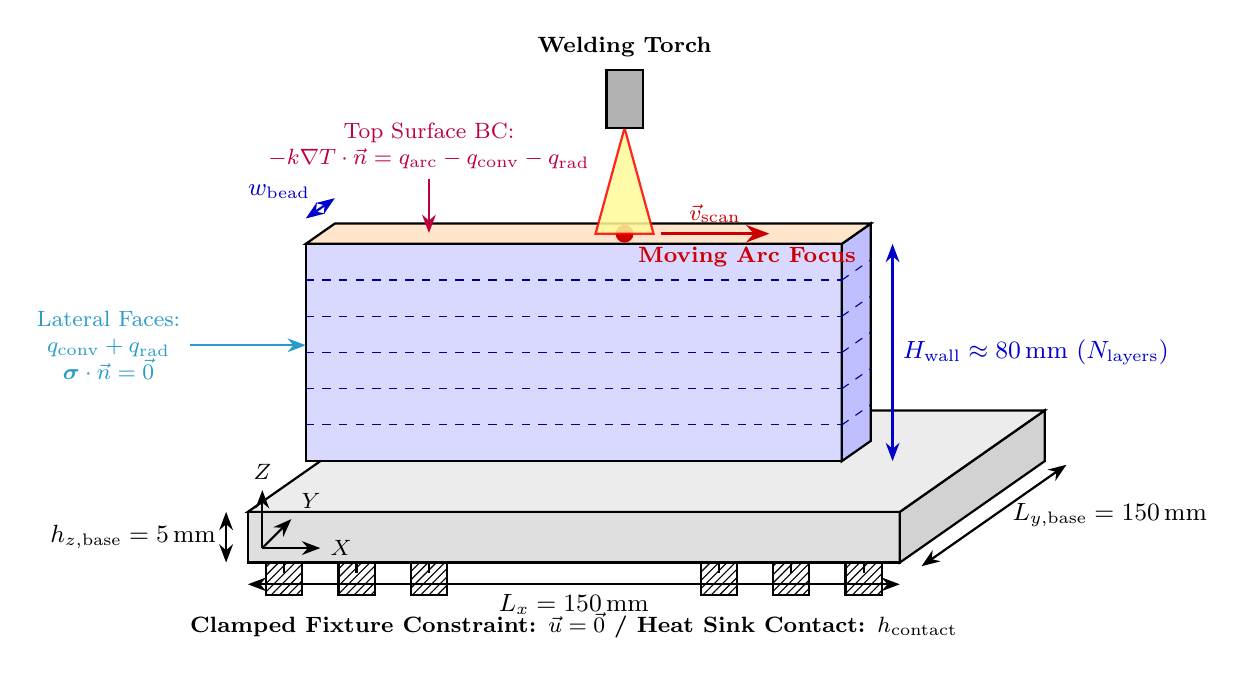
\begin{tikzpicture}[scale=0.92, >=Stealth, font=\small]
    % Coordinates for Baseplate
    \coordinate (B0) at (0, 0);
    \coordinate (B1) at (9.0, 0);
    \coordinate (B2) at (11.0, 1.4);
    \coordinate (B3) at (2.0, 1.4);
    
    \coordinate (T0) at (0, 0.7);
    \coordinate (T1) at (9.0, 0.7);
    \coordinate (T2) at (11.0, 2.1);
    \coordinate (T3) at (2.0, 2.1);
    
    % Draw Baseplate
    \draw[thick, fill=gray!25] (B0) -- (B1) -- (T1) -- (T0) -- cycle;
    \draw[thick, fill=gray!35] (B1) -- (B2) -- (T2) -- (T1) -- cycle;
    \draw[thick, fill=gray!15] (T0) -- (T1) -- (T2) -- (T3) -- cycle;
    
    % Baseplate Dimension Annotations
    \draw[<->, thick] (0, -0.3) -- (9.0, -0.3) node[midway, below] {$L_x = 150\,\mathrm{mm}$};
    \draw[<->, thick] (9.3, -0.05) -- (11.3, 1.35) node[midway, right=3pt] {$L_{y,\mathrm{base}} = 150\,\mathrm{mm}$};
    \draw[<->, thick] (-0.3, 0) -- (-0.3, 0.7) node[midway, left] {$h_{z,\mathrm{base}} = 5\,\mathrm{mm}$};

    % Coordinates for Deposited Wall (Centered in Y at Y = 75 mm)
    \coordinate (W_B0) at (0.8, 1.4);
    \coordinate (W_B1) at (8.2, 1.4);
    \coordinate (W_B2) at (8.6, 1.68);
    \coordinate (W_B3) at (1.2, 1.68);

    \coordinate (W_T0) at (0.8, 4.4);
    \coordinate (W_T1) at (8.2, 4.4);
    \coordinate (W_T2) at (8.6, 4.68);
    \coordinate (W_T3) at (1.2, 4.68);

    % Draw Deposited Wall
    \draw[thick, fill=blue!15] (W_B0) -- (W_B1) -- (W_T1) -- (W_T0) -- cycle;
    \draw[thick, fill=blue!25] (W_B1) -- (W_B2) -- (W_T2) -- (W_T1) -- cycle;
    \draw[thick, fill=orange!20] (W_T0) -- (W_T1) -- (W_T2) -- (W_T3) -- cycle;

    % Multi-layer horizontal stratification lines
    \foreach \y in {1.9, 2.4, 2.9, 3.4, 3.9} {
        \draw[thin, blue!60!black, dashed] (0.8, \y) -- (8.2, \y);
        \draw[thin, blue!60!black, dashed] (8.2, \y) -- (8.6, \y + 0.28);
    }
    
    % Wall Dimension Annotations
    \draw[<->, thick, blue!80!black] (8.9, 1.4) -- (8.9, 4.4) node[midway, right] {$H_{\mathrm{wall}} \approx 80\,\mathrm{mm}$ ($N_{\mathrm{layers}}$)};
    \draw[<->, thick, blue!80!black] (0.8, 4.75) -- (1.2, 5.03) node[midway, above left] {$w_{\mathrm{bead}}$};

    % Torch & Heat Source Representation
    \coordinate (Torch) at (5.2, 4.54);
    \fill[red!80!black] (Torch) circle (3.5pt) node[below right=2pt, font=\bfseries\footnotesize, red!80!black] {Moving Arc Focus};
    
    % Torch Cone
    \draw[thick, red, fill=yellow!40, opacity=0.85] (5.2, 6.0) -- (4.8, 4.54) -- (5.6, 4.54) -- cycle;
    \draw[thick, fill=gray!60] (4.95, 6.0) rectangle (5.45, 6.8);
    \node[above, font=\footnotesize\bfseries] at (5.2, 6.85) {Welding Torch};
    \draw[->, very thick, red!80!black] (5.7, 4.54) -- (7.2, 4.54) node[midway, above, font=\footnotesize\bfseries] {$\vec{v}_{\mathrm{scan}}$};

    % Boundary Condition Callouts
    \draw[->, thick, purple] (2.5, 5.3) -- (2.5, 4.55);
    \node[above, font=\footnotesize, purple, align=center] at (2.5, 5.3) {Top Surface BC:\\$-k\nabla T\cdot\vec{n} = q_{\mathrm{arc}} - q_{\mathrm{conv}} - q_{\mathrm{rad}}$};

    \draw[->, thick, cyan!80!black] (-0.8, 3.0) -- (0.8, 3.0);
    \node[left, font=\footnotesize, cyan!80!black, align=center] at (-0.8, 3.0) {Lateral Faces:\\$q_{\mathrm{conv}} + q_{\mathrm{rad}}$\\$\boldsymbol{\sigma}\cdot\vec{n} = \vec{0}$};

    % Clamping Mechanical BC at Substrate Bottom
    \foreach \x in {0.5, 1.5, 2.5, 6.5, 7.5, 8.5} {
        \draw[thick, pattern=north east lines] (\x - 0.25, -0.45) rectangle (\x + 0.25, 0);
        \draw[thick] (\x, 0) -- (\x, -0.15);
    }
    \node[below, font=\footnotesize\bfseries, align=center] at (4.5, -0.55) {Clamped Fixture Constraint: $\vec{u} = \vec{0}$ / Heat Sink Contact: $h_{\mathrm{contact}}$};

    % Coordinate System
    \draw[->, thick] (0.2, 0.2) -- (1.0, 0.2) node[right, font=\footnotesize] {$X$};
    \draw[->, thick] (0.2, 0.2) -- (0.6, 0.6) node[above right, font=\footnotesize] {$Y$};
    \draw[->, thick] (0.2, 0.2) -- (0.2, 1.0) node[above, font=\footnotesize] {$Z$};
\end{tikzpicture}
\caption{Three-dimensional computational domain schematic for the WAAM simulation showing: (i) solid substrate baseplate ($150\times 150\times 5\,\mathrm{mm}$); (ii) multi-layer deposited thin wall ($150\times w_{\mathrm{bead}}\times 80\,\mathrm{mm}$); (iii) moving welding torch travel along $\vec{v}_{\mathrm{scan}}$; (iv) thermal convective and radiative boundary conditions; and (v) baseplate mechanical clamping and thermal contact conductance.}
\label{fig:domain}
\end{figure}

\subsection{Single Bead Geometry and Longitudinal Goldak Source}
Figure~\ref{fig:bead} shows the transverse cross-section of a single deposited bead and the longitudinal profile of the Goldak double-ellipsoid heat source.

\begin{figure}[h!]
\centering
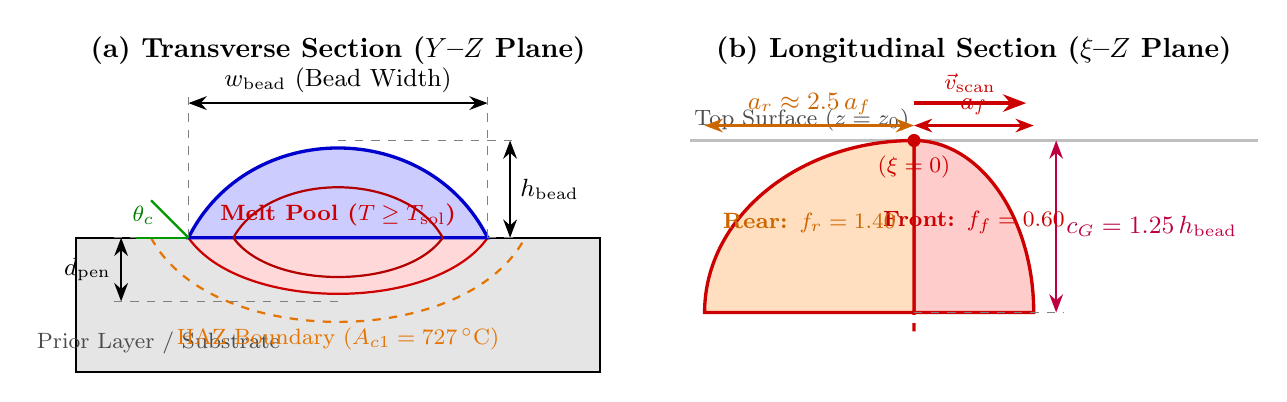
\begin{tikzpicture}[scale=0.95, >=Stealth, font=\small]
    % ----------------------------------------------------
    % (a) Transverse Cross-Section (Y-Z plane)
    % ----------------------------------------------------
    \begin{scope}[shift={(0,0)}]
        \node[font=\bfseries\normalsize] at (3.5, 4.3) {(a) Transverse Section ($Y$--$Z$ Plane)};
        
        % Substrate / Prior Layer Base
        \draw[thick, fill=gray!20] (0, 0) rectangle (7.0, 1.8);
        \node at (1.1, 0.4) [font=\footnotesize, gray!60!black] {Prior Layer / Substrate};

        % Fusion Line (Penetration into base)
        \draw[thick, red!80!black, fill=red!15] (1.5, 1.8) .. controls (2.2, 0.8) and (4.8, 0.8) .. (5.5, 1.8) -- cycle;
        
        % Deposited Parabolic Reinforcement
        \draw[very thick, blue!80!black, fill=blue!20] (1.5, 1.8) .. controls (2.3, 3.4) and (4.7, 3.4) .. (5.5, 1.8) -- cycle;
        
        % HAZ Boundary (Dotted)
        \draw[thick, orange!90!black, dashed] (1.0, 1.8) .. controls (1.8, 0.3) and (5.2, 0.3) .. (6.0, 1.8);
        \node[orange!90!black, font=\footnotesize] at (3.5, 0.45) {HAZ Boundary ($A_{c1} = 727\,^\circ\mathrm{C}$)};

        % Liquid Pool Isotherm (Solidus 1402 °C)
        \draw[thick, red!70!black] (2.1, 1.8) .. controls (2.6, 2.7) and (4.4, 2.7) .. (4.9, 1.8);
        \draw[thick, red!70!black] (2.1, 1.8) .. controls (2.6, 1.1) and (4.4, 1.1) .. (4.9, 1.8);
        \node[red!80!black, font=\bfseries\footnotesize] at (3.5, 2.1) {Melt Pool ($T \ge T_{\mathrm{sol}}$)};

        % Dimensions
        % Bead Width
        \draw[<->, thick] (1.5, 3.6) -- (5.5, 3.6) node[midway, above] {$w_{\mathrm{bead}}$ (Bead Width)};
        \draw[dashed, gray] (1.5, 1.8) -- (1.5, 3.7);
        \draw[dashed, gray] (5.5, 1.8) -- (5.5, 3.7);

        % Bead Height
        \draw[<->, thick] (5.8, 1.8) -- (5.8, 3.1) node[midway, right] {$h_{\mathrm{bead}}$};
        \draw[dashed, gray] (3.5, 3.1) -- (5.9, 3.1);
        \draw[dashed, gray] (5.5, 1.8) -- (5.9, 1.8);

        % Penetration Depth
        \draw[<->, thick] (0.6, 0.95) -- (0.6, 1.8) node[midway, left] {$d_{\mathrm{pen}}$};
        \draw[dashed, gray] (0.5, 1.8) -- (1.5, 1.8);
        \draw[dashed, gray] (0.5, 0.95) -- (3.5, 0.95);

        % Wetting Angle
        \draw[thick, green!60!black] (1.5, 1.8) -- (1.0, 2.3);
        \draw[thick, green!60!black] (1.5, 1.8) -- (0.8, 1.8);
        \node[green!50!black, font=\footnotesize] at (0.9, 2.1) {$\theta_c$};
    \end{scope}

    % ----------------------------------------------------
    % (b) Longitudinal Goldak Source (xi-Z plane)
    % ----------------------------------------------------
    \begin{scope}[shift={(8.2,0)}]
        \node[font=\bfseries\normalsize] at (3.8, 4.3) {(b) Longitudinal Section ($\xi$--$Z$ Plane)};

        % Top Surface Line
        \draw[thick, gray!50] (0, 3.1) -- (7.6, 3.1);
        \node[above, font=\footnotesize, gray!60!black] at (1.5, 3.1) {Top Surface ($z = z_0$)};

        % Goldak Double Ellipsoid
        % Center Arc Axis
        \coordinate (GC) at (3.0, 3.1);
        \draw[very thick, red!80!black, dashed] (GC) -- (3.0, 0.5);

        % Front Semi-Ellipsoid (xi >= 0, right side)
        \draw[very thick, red!80!black, fill=red!20] (3.0, 3.1) arc (90:0:1.6 and 2.3) -- (3.0, 0.8) -- cycle;
        % Rear Semi-Ellipsoid (xi < 0, left side, elongated)
        \draw[very thick, red!80!black, fill=orange!25] (3.0, 3.1) arc (90:180:2.8 and 2.3) -- (3.0, 0.8) -- cycle;

        % Semi-axes Dimensions
        % af (Front)
        \draw[<->, thick, red!80!black] (3.0, 3.3) -- (4.6, 3.3) node[midway, above] {$a_f$};
        % ar (Rear)
        \draw[<->, thick, orange!80!black] (0.2, 3.3) -- (3.0, 3.3) node[midway, above] {$a_r \approx 2.5\,a_f$};
        % cG (Depth)
        \draw[<->, thick, purple] (4.9, 0.8) -- (4.9, 3.1) node[midway, right] {$c_G = 1.25\,h_{\mathrm{bead}}$};
        \draw[dashed, gray] (3.0, 0.8) -- (5.0, 0.8);

        % Power partition labels
        \node[font=\bfseries\footnotesize, red!80!black] at (3.8, 2.0) {Front: $f_f = 0.60$};
        \node[font=\bfseries\footnotesize, orange!80!black] at (1.6, 2.0) {Rear: $f_r = 1.40$};

        % Travel Velocity
        \draw[->, very thick, red!80!black] (3.0, 3.6) -- (4.5, 3.6) node[midway, above, font=\footnotesize\bfseries] {$\vec{v}_{\mathrm{scan}}$};
        \fill[red!80!black] (GC) circle (2.5pt) node[below=2pt, font=\footnotesize] {$(\xi = 0)$};
    \end{scope}
\end{tikzpicture}
\caption{Detailed single bead schematic: (a) Transverse cross-section in the $Y$--$Z$ plane depicting parabolic bead reinforcement height $h_{\mathrm{bead}}$, bead width $w_{\mathrm{bead}}$, penetration depth $d_{\mathrm{pen}}$, wetting contact angle $\theta_c$, and the heat-affected zone (HAZ); (b) Longitudinal section in the $\xi$--$Z$ plane showing the moving Goldak double-ellipsoid core with front semi-axis $a_f$, rear semi-axis $a_r$, and depth $c_G$.}
\label{fig:bead}
\end{figure}

\subsection{Meshing Strategy and Single Cell Discretization}
Figure~\ref{fig:mesh} depicts the structured conforming multi-layer mesh along with a single 8-node hexahedral finite element cell showing nodal degrees of freedom, integration Gauss points, and the staggered coupling algorithm.

\begin{figure}[h!]
\centering
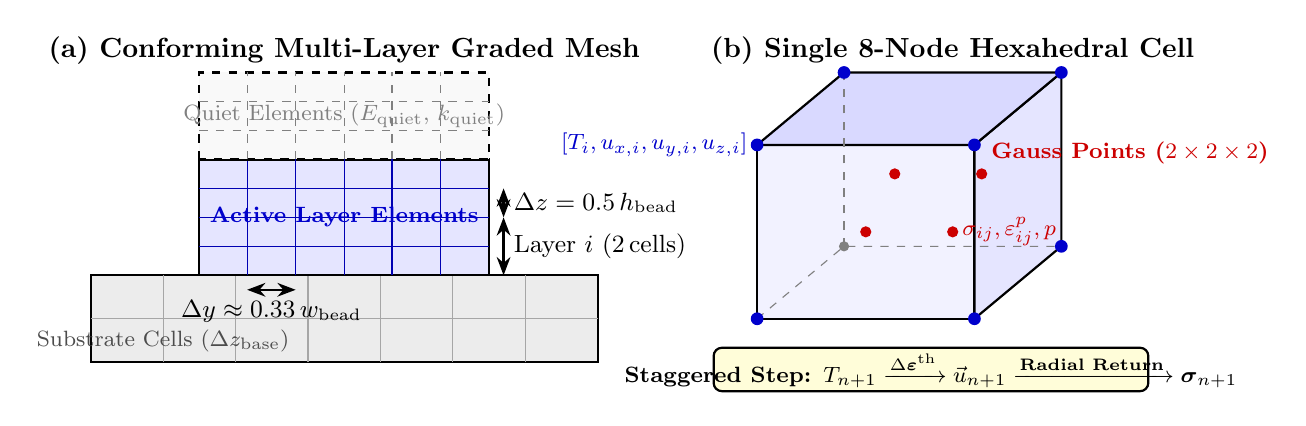
\begin{tikzpicture}[scale=0.92, >=Stealth, font=\small]
    % ----------------------------------------------------
    % (a) Multi-Layer Graded Mesh
    % ----------------------------------------------------
    \begin{scope}[shift={(0,0)}]
        \node[font=\bfseries\normalsize] at (3.5, 4.3) {(a) Conforming Multi-Layer Graded Mesh};

        % Substrate Mesh (Coarser)
        \draw[thick, fill=gray!15] (0, 0) rectangle (7.0, 1.2);
        \foreach \x in {1.0, 2.0, 3.0, 4.0, 5.0, 6.0} {
            \draw[gray!70] (\x, 0) -- (\x, 1.2);
        }
        \draw[gray!70] (0, 0.6) -- (7.0, 0.6);
        \node[font=\footnotesize, gray!60!black] at (1.0, 0.3) {Substrate Cells ($\Delta z_{\mathrm{base}}$)};

        % Deposited Fine Mesh (Layer 1 to Layer N)
        % Active Layers
        \draw[thick, fill=blue!10] (1.5, 1.2) rectangle (5.5, 2.8);
        \foreach \y in {1.6, 2.0, 2.4} {
            \draw[blue!70!black] (1.5, \y) -- (5.5, \y);
        }
        \foreach \x in {2.16, 2.83, 3.5, 4.16, 4.83} {
            \draw[blue!70!black] (\x, 1.2) -- (\x, 2.8);
        }
        \node[font=\bfseries\footnotesize, blue!80!black] at (3.5, 2.0) {Active Layer Elements};

        % Quiet / Inactive Elements (Dashed)
        \draw[thick, dashed, fill=gray!5] (1.5, 2.8) rectangle (5.5, 4.0);
        \foreach \y in {3.2, 3.6} {
            \draw[gray, dashed] (1.5, \y) -- (5.5, \y);
        }
        \foreach \x in {2.16, 2.83, 3.5, 4.16, 4.83} {
            \draw[gray, dashed] (\x, 2.8) -- (\x, 4.0);
        }
        \node[font=\footnotesize, gray] at (3.5, 3.4) {Quiet Elements ($E_{\mathrm{quiet}},\,k_{\mathrm{quiet}}$)};

        % Annotations
        \draw[<->, thick] (5.7, 1.2) -- (5.7, 2.0) node[midway, right] {Layer $i$ ($2\,\text{cells}$)};
        \draw[<->, thick] (5.7, 2.0) -- (5.7, 2.4) node[midway, right] {$\Delta z = 0.5\,h_{\mathrm{bead}}$};
        \draw[<->, thick] (2.16, 1.0) -- (2.83, 1.0) node[midway, below] {$\Delta y \approx 0.33\,w_{\mathrm{bead}}$};
    \end{scope}

    % ----------------------------------------------------
    % (b) Single Hexahedral FE Cell (8-node, Gauss Points)
    % ----------------------------------------------------
    \begin{scope}[shift={(8.4,0)}]
        \node[font=\bfseries\normalsize] at (3.5, 4.3) {(b) Single 8-Node Hexahedral Cell};

        % Hexahedral Vertices
        \coordinate (N1) at (0.8, 0.6);
        \coordinate (N2) at (3.8, 0.6);
        \coordinate (N3) at (5.0, 1.6);
        \coordinate (N4) at (2.0, 1.6);

        \coordinate (N5) at (0.8, 3.0);
        \coordinate (N6) at (3.8, 3.0);
        \coordinate (N7) at (5.0, 4.0);
        \coordinate (N8) at (2.0, 4.0);

        % Draw Hexahedron
        \draw[thick, fill=blue!5] (N1) -- (N2) -- (N6) -- (N5) -- cycle;
        \draw[thick, fill=blue!10] (N2) -- (N3) -- (N7) -- (N6) -- cycle;
        \draw[thick, fill=blue!15] (N5) -- (N6) -- (N7) -- (N8) -- cycle;
        \draw[dashed, gray] (N1) -- (N4) -- (N3);
        \draw[dashed, gray] (N4) -- (N8);

        % Nodes
        \foreach \p in {N1, N2, N3, N5, N6, N7, N8} {
            \fill[blue!80!black] (\p) circle (2.5pt);
        }
        \fill[gray] (N4) circle (2.0pt);

        % Nodal DOFs Callout
        \node[left, font=\footnotesize, blue!80!black] at (N5) {$[T_i, u_{x,i}, u_{y,i}, u_{z,i}]$};

        % Gauss Points (2x2x2 Integration Points)
        \coordinate (GP1) at (2.3, 1.8);
        \coordinate (GP2) at (3.5, 1.8);
        \coordinate (GP3) at (2.7, 2.6);
        \coordinate (GP4) at (3.9, 2.6);
        
        \foreach \g in {GP1, GP2, GP3, GP4} {
            \fill[red!80!black] (\g) circle (2.2pt);
        }
        \node[above right, font=\footnotesize\bfseries, red!80!black] at (GP4) {Gauss Points ($2\times 2\times 2$)};
        \node[right, font=\footnotesize, red!80!black] at (GP2) {$\sigma_{ij}, \varepsilon^p_{ij}, p$};

        % Coupling Workflow Banner Below Cell
        \draw[thick, fill=yellow!15, rounded corners=3pt] (0.2, -0.4) rectangle (6.2, 0.2);
        \node[font=\footnotesize\bfseries, align=center] at (3.2, -0.1) {Staggered Step: $T_{n+1} \xrightarrow{\Delta\boldsymbol{\varepsilon}^{\mathrm{th}}} \vec{u}_{n+1} \xrightarrow{\text{Radial Return}} \boldsymbol{\sigma}_{n+1}$};
    \end{scope}
\end{tikzpicture}
\caption{Finite element meshing strategy: (a) Multi-layer graded mesh illustrating structured element rows ($\Delta z = 0.5\,h_{\mathrm{bead}}$), transverse sizing ($\Delta y = 0.25\text{--}0.33\,w_{\mathrm{bead}}$), and inactive quiet elements; (b) Single hexahedral finite element ($8$-node) showing nodal degrees of freedom $[T_i, u_{x,i}, u_{y,i}, u_{z,i}]$, Gauss quadrature integration points, and the staggered coupling workflow.}
\label{fig:mesh}
\end{figure}

\section{Conclusion}
This report has codified the complete continuum mechanics formulations, spatial meshing strategies, Goldak heat source parameterization rules, and boundary condition matrices implemented in our FreeFEM++ WAAM framework. By eliminating empirical assumptions and grounding mesh sizing ($\Delta z = 0.5\,h_{\mathrm{bead}}$, $\Delta y = 0.33\,w_{\mathrm{bead}}$), heat source dimensions ($b_G = 0.5\,w_{\mathrm{bead}}$, $c_G = 1.25\,h_{\mathrm{bead}}$), and quiet element stabilization in rigorous physical conservation principles, the framework provides predictive fidelity across varied currents, voltages, and wire travel velocities.

\vspace{1.0em}
\noindent\rule{0.4\textwidth}{0.4pt}\par
\vspace{0.2em}
\noindent\small\textit{Report compiled on October 13, 2026. Prepared for academic submission and review at the Indian Institute of Space Science and Technology (IIST), Thiruvananthapuram.}

\end{document}
